\documentclass{article}
\title{OS Lab Report IV}
\usepackage{fullpage}
\usepackage{array}
\usepackage{multicol}
\usepackage{listings}
\usepackage{graphicx}

\begin{document}
\newcommand{\incell}[1]{\begin{tabular}{c}#1\end{tabular}}
%\maketitle
\begin{center}
\LARGE{OS Lab Report IV}
\end{center}
\begin{center}
\begin{tabular}{cc}
\incell{10152130255\\Lv Yingzhe}&
\incell{10152130134\\Yao Shunyu}
\end{tabular}
\end{center}
\vspace{2em}


\section{Introduction}
In this project, we implemented a variety of locks, and built some concurrent data structures like counter, linked-list and hash-list based on our locks. After that, we do performance and fairness tests to analyze different lock implements. By doing so, we got a sense of lock primitives, parallel mechanism and programming technique.


\section{Lock Implementation}
In this section, we will discuss locks (and synchronization device, specifically, we mean condition variable) we implemented. Except obligate spin-lock and mutex required by the specification, we also implemented other fancy locks like: two-phase lock, mixing spin-lock and mutex, trying not to fall into kernel mode to improve lock performance, and read-write lock, parallelize read requests for the critical section to improve performance. Introduction of our locks are listed as below:
\begin{center}
\begin{tabular}{c|l|c}
\hline
Lock Type& \multicolumn{1}{c|}{Interface}& Description\\
\hline
Spin-lock&
\begin{lstlisting}
spinlock_init(lock);
spinlock_acquire(lock);
spinlock_release(lock);
\end{lstlisting}
& Simply busy-waiting\\
\hline
Mutex& 
\begin{lstlisting}
mutex_init(lock);
mutex_acquire(lock);
mutex_release(lock);
\end{lstlisting}
& Sleep and wake using futex\\
\hline
Two-phase&
\begin{lstlisting}
twophase_init(lock);
twophase_acquire(lock);
twophase_release(lock);
\end{lstlisting}
& Hybrid of spin-lock and mutex\\
\hline
\incell{Condition\\Variable}&
\begin{lstlisting}
cond_init(cv);
cond_wait(cv, mutex);
cond_signal(cv);
cond_broadcast(cv);
\end{lstlisting}
& Synchronization device on a predicate\\
\hline
Read-write lock&
\begin{lstlisting}
rwlock_init(lock);
rwlock_rdlock(lock);
rwlock_wrlock(lock);
rwlock_unlock(lock);
\end{lstlisting}
& Support concurrent read requests\\
\hline
\end{tabular}
\end{center}

\subsection{Spin Lock}
Spin-lock is the most simply lock implementation, what it does is keeping trying to acquire the lock in a loop. The only technique required is to check the condition and set it simultaneously, which intend to avoid synchronize problems like multiple access caused by context switch. Fortunately, Intel x86 machine support an instruction \textbf{xchg} to complete this work.

\subsection{Mutex}
Mutex is another implementation of lock which causes threads to sleep rather than just spin when the lock is unavailable to spare CPU from blocking threads. We won't implement waiting queue and wait/wake mechanism since Linux provides the system calls named \textbf{futex} for this purpose (additionally, trying to implement a queue in user mode will cause unpredictable problems, like send a signal to some completely wrong thread, personally, I'm against this approach).

\subsection{Two-phase Lock}
The two-phase lock is designed to maximally reduce the cost of thread sleep/wake, as a result improve the lock performance. The idea of two-phase lock based on the truth that a great amount of critical sections are short, if a thread directly go to sleep once it can't acquire the lock, it may lost the chance acquiring lock released after a very short time.\\
On the acquire end, threads trying to acquire the lock in a loop for a period of time in the first phase (like spin-lock do, except it can get out of the loop after a few attempts using \textbf{cmpxchg}). If it still blocked after that, it will sleep as mutex do. On the release end, threads also get into spin loop phase, trying to give the lock to a waiting thread in the first phase. If failed, it will wake up a sleeping thread.\\
We must notice that the loop time in the first phase is determined by the programmer, so it's a hard quest to set a proper loop time to maximize performance.

\subsection{Condition Variable}
A condition variable is a synchronization construct that allows threads to have both mutual exclusion and the ability to wait for a certain condition to become true. It have a mechanism for signaling other threads that their condition has been met (cond signal or cond broadcast), also provides a mechanism for threads to temporarily give up exclusive access in order to wait for some condition to be met, before regaining exclusive access and resuming their task (cond wait).\\
Note that condition variable is a kind of synchronization device, NOT a lock. We implement this gadget mainly to pave the way for read-write lock. What makes it different from locks is that it provides an effective method to wake up all waiting threads. It's also a useful tool in multi-thread programming if you wish.

\subsection{Read-write Lock}
Considering the high frequency of read requests to the critical section, forcing all request (include reading request) serialized is unacceptable on performance, that's why we implemented read-write lock in this project.\\
A read-write lock a synchronization primitive that allows concurrent access for read-only operations, while write operations require exclusive access. This means that multiple threads can read the data in parallel but an exclusive lock is needed for writing or modifying data. When one writer is writing the data, all other writers or readers will be blocked until the writer is finished writing.\\
We implement the read-write lock on the basis of condition variable for performance consideration. Just imagine there are many readers waiting on a read-write lock, and a writer just completed its work and ready to release the lock. If we use futex wake to wake these threads, then readers all awaken, trying to acquire mutex, and sleep again except the lucky one who acquired the lock. Such a phenomenon is called \textbf{thundering herd}, will cause unintended cost of context switch. To avoid that, we use condition variable to requeue all waiting readers on the mutex waiting queue except one thread, which will be waken.


\section{Library Implementation}
We also build some concurrent data structures on the locks we implemented. Note that we don't implement any error check to make performance tests more accurate. These implements are very simple, so we only list all interfaces:
\begin{center}
\begin{tabular}{c|l}
\hline
Library&\multicolumn{1}{c}{Interface}\\
\hline
Concurrent counter&
\begin{lstlisting}
void counter_init(counter_t *c, int value);
int counter_get_value(counter_t *c);
void counter_increment(counter_t *c);
void counter_decrement(counter_t *c);
\end{lstlisting}\\
\hline
Concurrent List&
\begin{lstlisting}
void list_init(list_t *list);
void list_insert(list_t *list, unsigned int key);
void list_delete(list_t *list, unsigned int key);
void *list_lookup(list_t *list, unsigned int key);
long long list_sum(list_t *list);
int list_count(list_t *list);
void list_destroy(list_t *list);
\end{lstlisting}\\
\hline
Concurrent Hash&
\begin{lstlisting}
void hash_init(hash_t *hash, int size);
void hash_insert(hash_t *hash, unsigned int key);
void hash_delete(hash_t *hash, unsigned int key);
void *hash_lookup(hash_t *hash, unsigned int key);
void hash_destroy(hash_t *hash);
\end{lstlisting}\\
\hline
\end{tabular}
\end{center}


\section{Performance}
What we must inform is that we run test program on a 4-core CPU computer, running a program with threads more than $4$ may cause great amount of context switch cost.
\subsection{Lock Comparison}
We firstly approximately test lock performance. This test is based on our \textbf{counter} implements, each thread increment a shared counter max times, the results are shown below:
\begin{center}
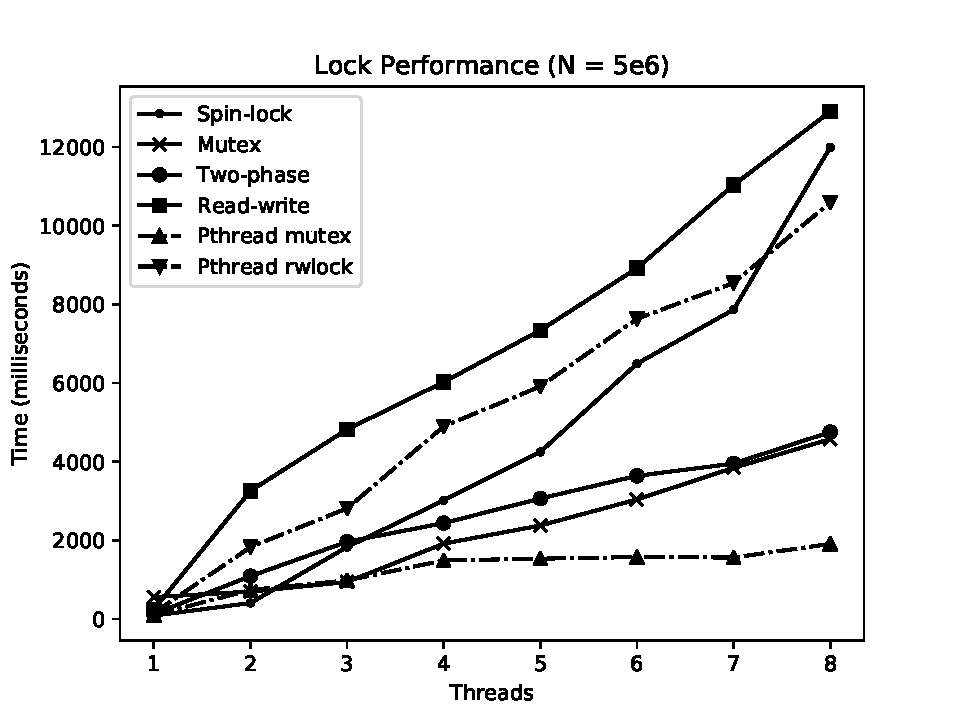
\includegraphics[height=24em]{OSLAB4_LOCK1.pdf}
\end{center}
\newpage

\begin{center}
\centerline{Lock Analysis}
\begin{tabular}{c|p{0.75\columnwidth}}
\hline
Spin-lock&
We notice that the spin-lock execution time increased most quickly, run most fast when only a few threads while run very slow when there're many threads. We assume when there are less than $4$ threads, each thread can take up a CPU core, so busy-waiting will not cause performance problem while no sleep and wake will reduce system call cost, while the thread number increasing, a busy-waiting core still take CPU resource but do nothing, that cause performance loss.\\
\hline
Mutex&
Mutex perform bad at beginning due to system call of futex, while perform well when there are more threads, since it can switch between threads to make good use of CPU.\\
\hline
Two-Phase&
Two-phase lock merging both the spin-lock and mutex advantage, so run faster than mutex at beginning and also faster that spin-lock after that.\\
\hline
Read-Write&
Read-write lock is \textbf{not designed for such use}, so it performs worst. We won't display read-write locks for the following write-only situations.\\
\hline
Pthread Mutex&
Pthread mutex performs awfully good, no matter thread number is big or small, Unix must have payed great effort to optimize it!\\
\hline
Pthread Read-Write&
Pthread read-write lock like our read-write lock implement, also perform bad in such situation.\\
\hline
\end{tabular}
\end{center}
We notice that the spin-lock execution time increased most quickly, run most fast when only a few threads while run very slow when there're many threads

\subsection{Two-Phase Argument}
Not mentioned previously, we set two-phase lock loop count to $100$, the reason can be simply inferred from the following graph:\\
\begin{center}
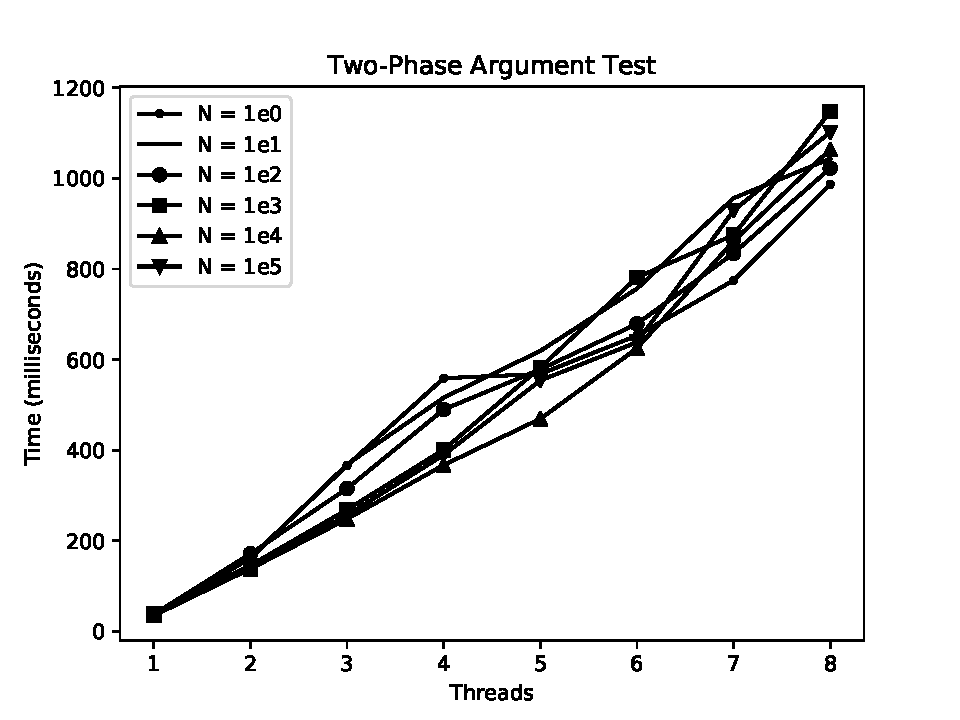
\includegraphics[height=24em]{OSLAB4_ARG.pdf}
\end{center}
The $6$ sampling we set have similar result, we choose $N=100$ because it have the most stable performance.

\subsection{List Performance}
In this section, we test our list implementation in three different manner. The first test insert into a shared list at max times then execute delete at max times (N=5e4), the second test randomly insert or delete a number from the list (N=2e6), the third test randomly lookup, insert or delete on the list (N=5e4), to compare with read-write lock on performance.
\begin{center}
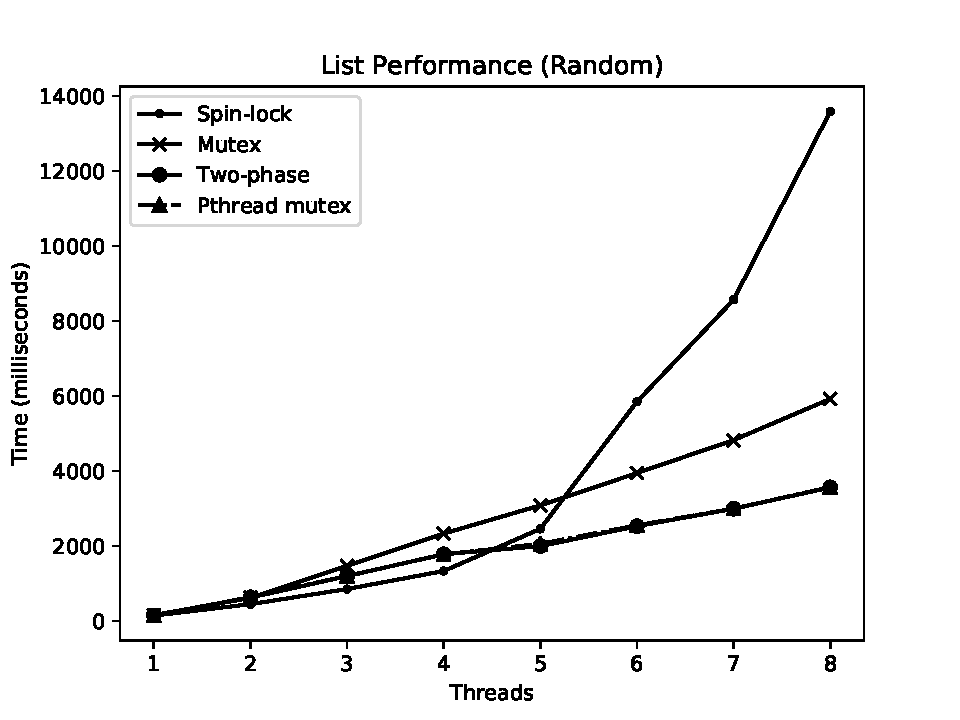
\includegraphics[width=0.65\textwidth]{OSLAB4_LIST1.pdf}
\end{center}
From this figure, we can found that spin-lock performs bad and obey the pattern we concluded in lock analysis part. The mutex lock, as a primitive lock implementation, also performs bad, but have a steady line, which means it's quite stable. The most interesting part is that our two-phase implementation and pthread mutex shared an almost same pattern, we guess in this situation, pthread mutex apply an approach just like our two-phase lock.
\begin{center}
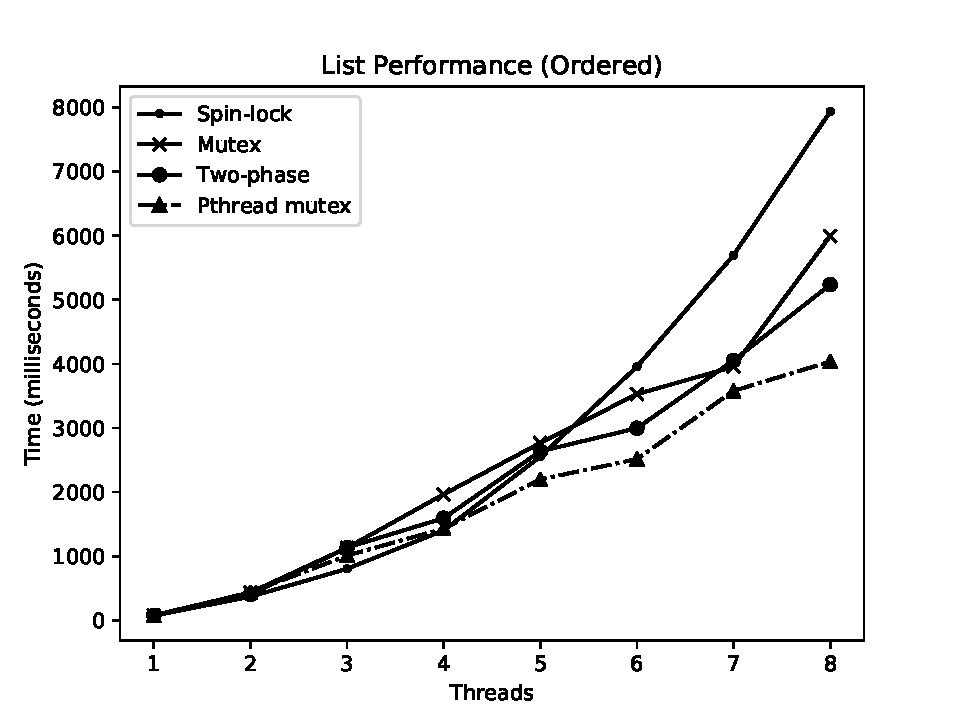
\includegraphics[width=0.65\textwidth]{OSLAB4_LIST2.pdf}
\end{center}
In this figure, spin-lock also performs as we predicted, while pthread mutex run faster than our two-phase lock this time, and mutex now performs similar to two-phase lock.
\begin{center}
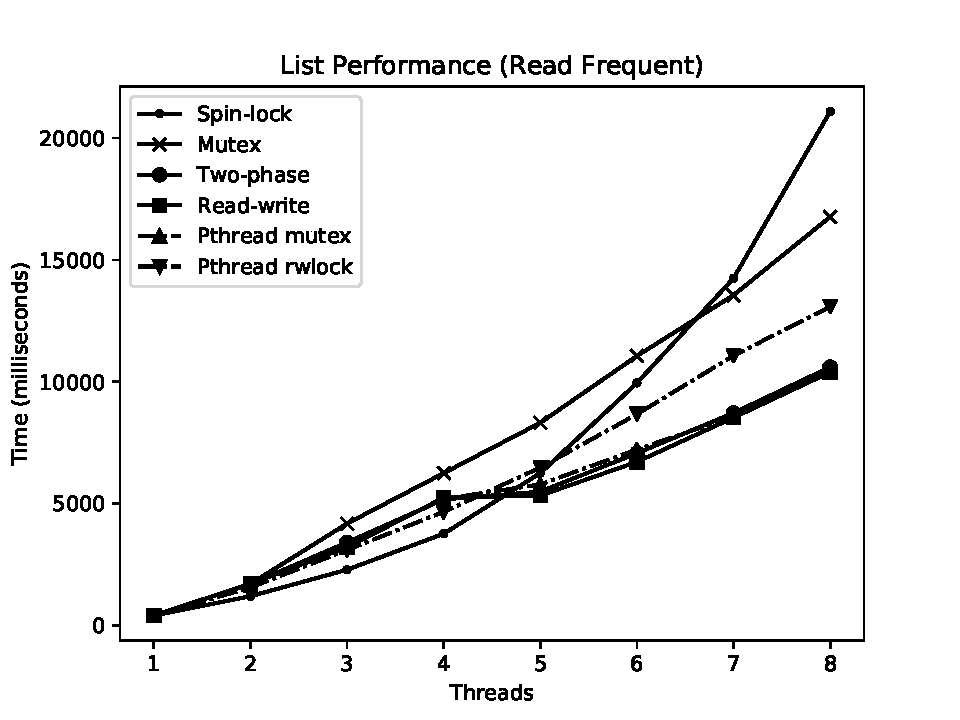
\includegraphics[width=0.65\textwidth]{OSLAB4_LIST3.pdf}
\end{center}
We use $70$ percent reading, $15$ percent inserting and $15$ percent deleting to simulate real situation. What we can find is that our read-write lock runs as fast as pthread mutex and two-phase lock, even faster than pthread read-write lock. Just as the previous two figures, mutex and spin-lock performs bad.

\subsection{Hash Performance}
The tests executed on hash is similar to list, except that all operations are executed on a hash instead of a list. The data scales are same as list.
\begin{center}
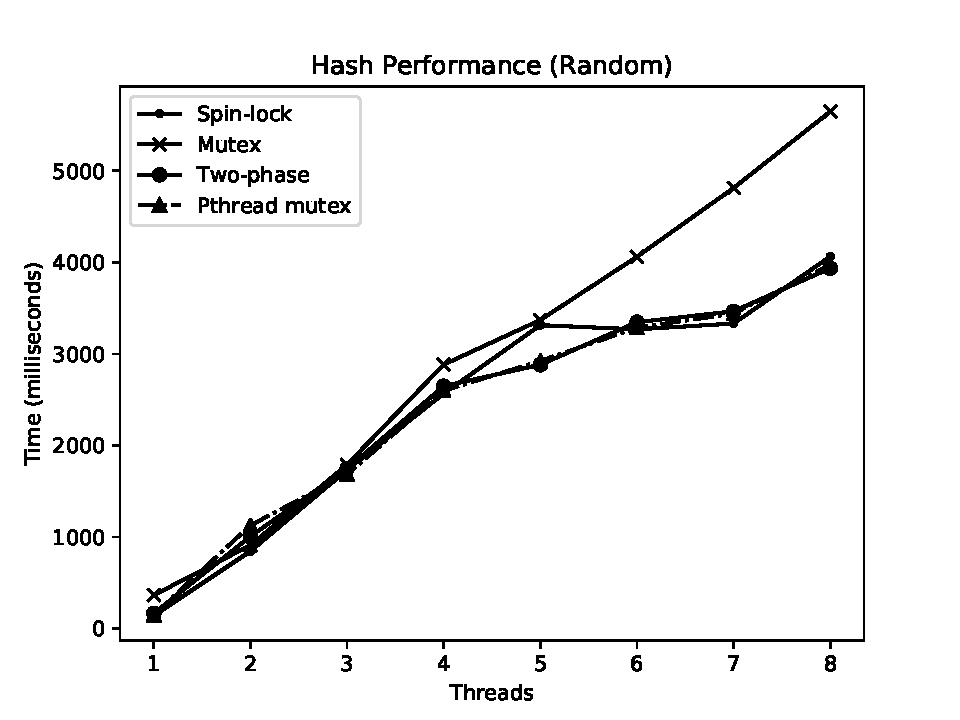
\includegraphics[width=0.65\textwidth]{OSLAB4_HASH1.pdf}
\end{center}
We can find the great power of hashing in this figure, since hash list let randomized request go into different lists, there are few access collision, so we can found that the execution time increases very slow after 4 threads except mutex. The bad performance of mutex may also caused by frequent kernel trap.
\begin{center}
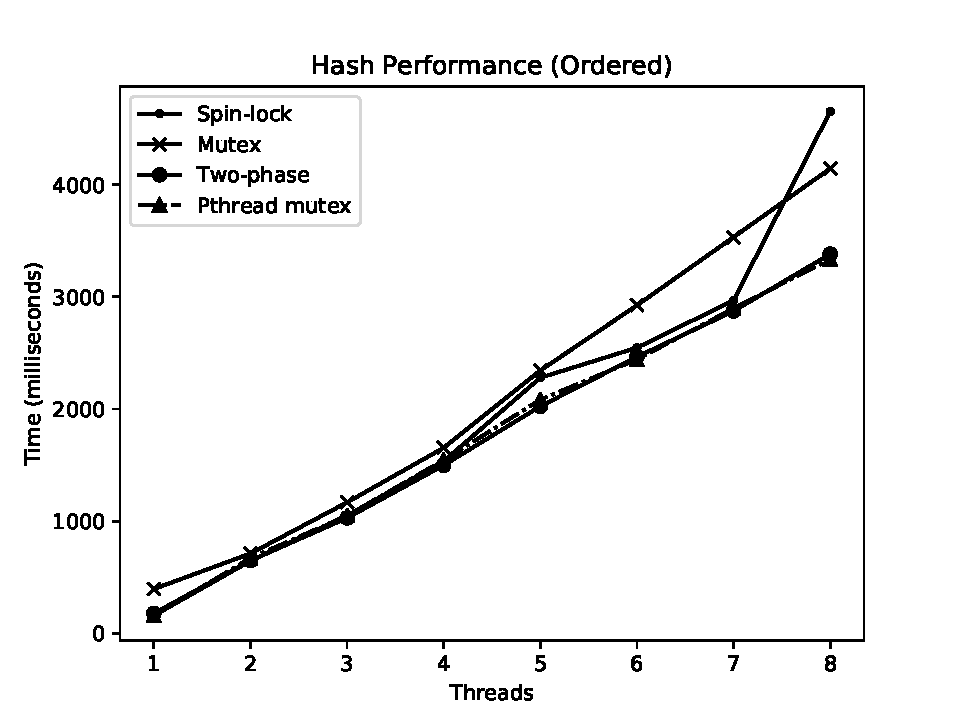
\includegraphics[width=0.65\textwidth]{OSLAB4_HASH2.pdf}
\end{center}
In this test, the insert and delete is executed in order, so the collision increased, and the performance is just the same as ordered list performance test.
\begin{center}
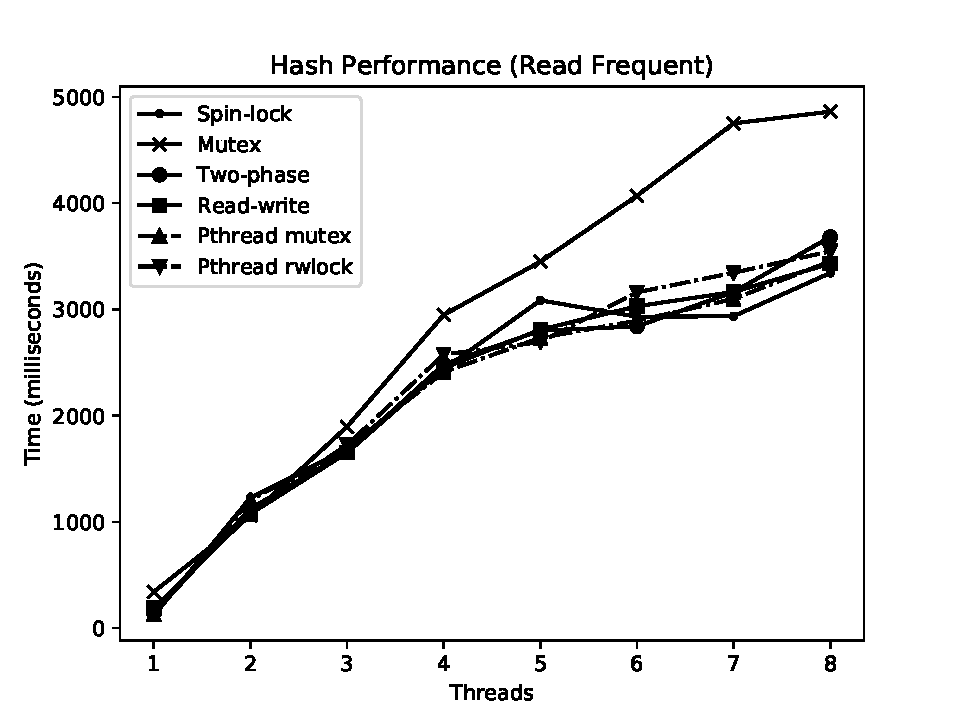
\includegraphics[width=0.65\textwidth]{OSLAB4_HASH3.pdf}
\end{center}
This test, again, is the show-time of read-write lock, it performs well, just like we mentioned in list part.

\subsection{Fairness Analysis}
The test of fairness is a head-scratching problem, since trying to measure lock acquire/release time will certainly cause \textbf{probe effect}, which means, unintended alternation will be introduced. We finally decided to use statistical sampling to reduce the affect of probing. Specifically, we calculation the derivation of \textbf{median time of reacquire} and \textbf{median time of execution} on different threads to judge the fairness of locks.\\
The measure we used in tests is \textbf{coefficient of variation (CV)}, also known as relative standard deviation, is a standardized measure of dispersion of a probability distribution or frequency distribution. It's definition is $CV=\frac{\sigma}{\mu}$, where $\sigma$ is the standard deviation and $\mu$ is the mean.
\begin{center}
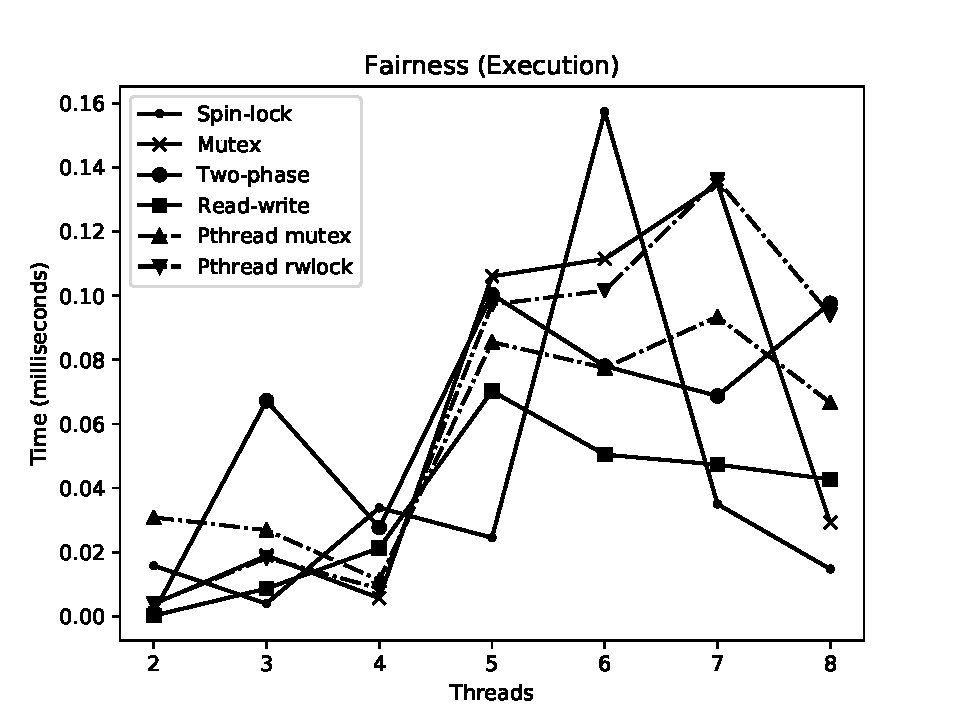
\includegraphics[width=0.65\textwidth]{OSLAB4_FAIR1.pdf}
\end{center}
\begin{center}
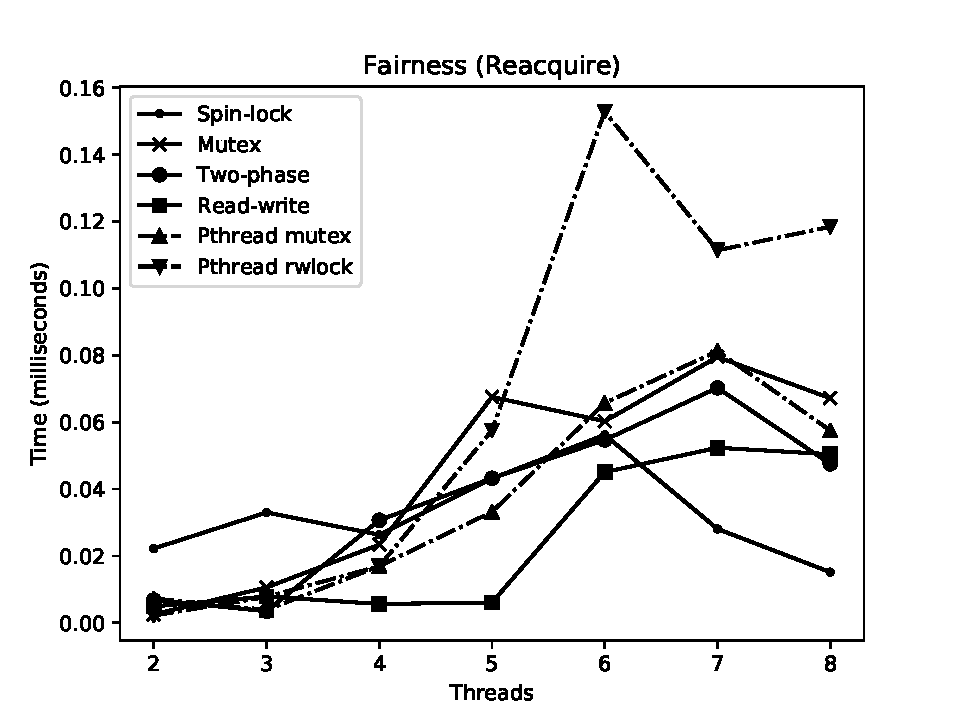
\includegraphics[width=0.65\textwidth]{OSLAB4_FAIR2.pdf}
\end{center}
From the two tests, we found that \textbf{in a short period}, all the locks can be treated as fair. We also noticed that pthread read-write lock not guarantee on fairness, and actually its variation is greatest. Interestingly, our read-write lock, in contrast, have the highest fairness.

\section{Summary}
We now conclude lock performance:
\begin{center}
\begin{tabular}{c|p{0.75\columnwidth}}
\hline
Spin-lock&
The spin-lock, as a busy-waiting implementation, perform well in situations when thread number less than CPU cores, or when collision is not serious. But due to its waste of CPU, it performs extremely bad on other situations.\\
\hline
Mutex&
Mutex is a very primitive lock type, since it frequently trapped into kernel, the cost of context switch is scalable, that's why it performs bad than other locks.\\
\hline
Two-Phase&
Two-phase lock merging both the spin-lock and mutex advantage, making it compatible in almost all situations. Personally, I think it can used to replace mutex.\\
\hline
Read-Write&
Read-write lock is designed for read-heavy mission, the performance is pretty well in such situation, but its cost is big in other situations. So use read-write or not, need an application programmer wisely judge.\\
\hline
\end{tabular}
\end{center}
We also notice that, hashing is powerful in balancing work. Even the simplest module hashing used in this project can greatly reduce access collision of critical sections.\\ Another important knowledge we got in this project is that, \textbf{pre-defined compiler macros} are quite useful! Without them, we may need one more day to modify code to complete all the tests.
\end{document}